% ===== 原文印刷页 127（PDF p.128）=====

\subsubsection{群的可积最高权表示} % 原文: 4.5.2 Integrable Highest Weight Representations Of The Group

{\small\itshape ［原文标记：一行星号分隔线］}
% [原文待办标记，原文 p.127；作者在标题下用一整行星号把"待写段落"与正文隔开]

\textbf{注记：}

\begin{itemize}
  \item 这些表示之所以称为可积的（integrable），是因为它们正是那些可以扩充为 $\widetilde{LG}$ 的表示。的确，它们是 $\widetilde{LG}$ 的幺正表示。此外，Borel-Weil 理论可以延拓到这个无穷维情形：$\widetilde{LG}/T$ 是一个无穷维复流形，$\widetilde{LG}/T\cong\widetilde{LG}_{\mathbb{C}}/B$，其中 $B$ 由那些可以全纯地延拓进圆盘的回圈组成。$LG/T$ 也是一个无穷维相空间，而该相空间的几何量子化给出 $\widetilde{LG}$ 的不可约表示。回圈群的 Borel-Weil 理论从数学角度在 Pressley-Segal 中有系统的发展。物理文献中同样有路径积分的处理。参见 ????。
\end{itemize}
% [原文待办标记，原文 p.127；"See ????" 是作者尚未填写的文献引用占位符，照原样保留]

{\small\itshape ［原文标记：又一行星号分隔线］}
% [原文待办标记，原文 p.127]

设 $G$ 单且紧。上文构造的中心扩张回圈群，对 $k\in\mathbb{Z}_+$ 将简记为 $G_k$。\footnote{一般地，对紧群可以证明，中心荷应当看作 $H^4(BG;\mathbb{Z})$ 的一个元素。当 $G$ 单、紧且连通时，这个上同调群同构于 $\mathbb{Z}$，于是我们可以把中心扩张看作一个整数。}

关于 $G_k$ 的表示我们能说些什么？显然有很多。例如，$G_k$ 有一个同态像 $LG$，因此，取 $G$ 的任一表示 $\rho:G\to\operatorname{Aut}(V)$（例如 $G$ 的一个有限维不可约表示）以及圆周上的一点 $z_0$，我们就可以定义求值表示（evaluation representation）：
\begin{equation}
  \widehat{\rho}: G_k \to \rho(g(z_0))
  \tag{4.147}
  \label{eq:4.147}
\end{equation}
其承载空间为 $V$。注意这些表示与 $L_0$ 相处得并\underline{不}好，因为 $L_0$ 会把 $z_0$ 平移成 $z_0e^{i\theta}$。

事实表明，$G_k$ 只有\underline{有限}多个 $L_0$ 有下界的不可约表示。这些表示自然地构造为 Lie 代数的最高权表示，并被称为\emph{可积表示}（integrable representations），因为它们能从 Lie 代数的表示扩充为 Lie 群的表示。

可积表示按 $L_0$ 分次，且谱有下界。$L_0$ 下的最低权空间本身是 $G$ 的一个不可约表示，它具有一个最高权 $\lambda$，对应于
\begin{equation}
  \Lambda_{wt}/W
  \tag{4.148}
  \label{eq:4.148}
\end{equation}
中的一个元素；其中 $W$ 是 Weyl 群，$\Lambda_{wt}$ 是权格。选定 $\mathfrak{g}$ 的一组单根之后，$G$ 的不可约表示的最高权可以用一个优势最高权（dominant highest weight）$\lambda\in\Lambda_{wt}$ 来标记。回忆这意味着
\begin{equation}
  \lambda=\sum n_i\lambda^{(i)}
  \tag{4.149}
  \label{eq:4.149}
\end{equation}
其中 $n_i\ge0$，而 $\lambda^{(i)}$ 是与单根对偶的一组基本权基。
% [Tutor Note: (4.148) 写的是商 $\Lambda_{wt}/W$，即最高权的 $W$-轨道；但紧接着又把 $\lambda$ 取成 $\Lambda_{wt}$ 中的优势权，这是选定了轨道在基本 Weyl 腔内的那个代表元，两者并不矛盾。另须分清三个格：权格 $\Lambda_{wt}$、余根格 $\Lambda_{crt}$（下一句 (4.151) 中仿射 Weyl 群的平移部分用它）、以及 $\Lambda_{weight}$（第 130 页起用以强调"权"的写法）；原文在不同页上用不同记号指同一个权格。]

% ===== 原文印刷页 128（PDF p.129）=====

现在看 $G_k$ 的情形：其不可约表示由商
\begin{equation}
  \Lambda_{wt}/\widehat{W}^{(k)}
  \tag{4.150}
  \label{eq:4.150}
\end{equation}
标记，其中 $\widehat{W}^{(k)}$ 是能级 $k$ 的仿射 Weyl 群。它是 $\mathrm{t}^\vee$ 的仿射变换群的一个离散晶体子群（crystallographic subgroup）。作为群，它同构于 Weyl 群 $W$ 与"沿余根格 $\Lambda_{crt}$ 的平移群"的半直积，但我们把它记作 $\widehat{W}^{(k)}$，因为这些平移的作用方式是
\begin{equation}
  \{\sigma|v\}: \lambda\mapsto \sigma(\lambda)+kv \qquad \sigma\in W,\ v\in\Lambda_{crt}
  \tag{4.151}
  \label{eq:4.151}
\end{equation}
% [Tutor Note: (4.151) 中能级 $k$ 只通过平移部分 $\sigma(\lambda)+kv$ 进入作用；这与"带移动"（shifted）的作用 $\lambda\mapsto\sigma(\lambda+\rho)-\rho$ 相差一个平移，后者的平移步长是 $k+h^\vee$（$h^\vee$ 为对偶 Coxeter 数，$SU(2)$ 时 $h^\vee=2$）。后文 (4.169) 里的 $k+2$ 与 (4.179) 的 $q=\exp\big(2\pi i/(k+h)\big)$ 都来自这种 shift，核算时务必分清 $k$ 与 $k+h^\vee$，否则 $S$ 矩阵 (4.175) 的归一化因子会差一个 $h^\vee$。]

值得知道的是，这是一个由反射生成的 Coxeter 群。这些反射包括 Weyl 反射，以及关于超平面 $(\lambda,\theta)=k$ 的反射；这里 $k\in\mathbb{Z}_+$，$\theta$ 是最高根，而我们采用使 $(\theta,\theta)=2$ 的 Killing 型归一化。该作用在 $\Lambda_{wt}$ 中的一个基本腔（fundamental chamber）是满足下述条件的优势权所成的有限集：
\begin{equation}
  (\lambda,\theta)\le k
  \tag{4.152}
  \label{eq:4.152}
\end{equation}
这个条件在共形场论中通常借助幺正性和零向量（null-vector）来导出。
% [Tutor Note: 作者略去了 (4.152) 的推导。被省略的中间步骤是：在能级 $k$ 的 Verma 模中显式构造相应能级的零向量（singular vector），要求它在物理态空间中被商掉，等价于该零向量的模方非负定；这正是 Kac-Kazhdan 可约性判别在 $\widehat{su}(2)$ 上的特例。具体计算见 Di Francesco、Mathieu、Sénéchal 书第 14 章，或 Kac 的《Infinite Dimensional Lie Algebras》第 11--12 章。]

\textbf{例 1}\quad $G=SU(2)$。此时 $\theta=\alpha$ 且 $\lambda=j\alpha$，其中 $j\in\frac12\mathbb{Z}_+$ 在物理中称为自旋。（数学家通常会写 $\lambda=n_1\lambda^{(1)}$，其中 $\lambda^{(1)}=\frac12\alpha_1$ 是基本权。于是 $n_1=2j$，是自旋的两倍。）$SU(2)$ 的、权为 $\lambda=j\alpha_1$ 的不可约表示的维数为 $2j+1$。格 $\Lambda_{wt}$ 同构于 $\mathbb{Z}$。$\mathrm{t}^\vee\cong\mathbb{R}$ 中的超平面是 $(x\alpha,\alpha)=k$，即 $x=k/2$。因此关于该超平面的反射把 $j$ 送到 $\frac{k}{2}-j$。所以仿射 Weyl 群的一个基本区域是：
\begin{equation}
  0\le j\le\frac{k}{2}
  \tag{4.153}
  \label{eq:4.153}
\end{equation}
注意此时 $\widehat{W}^k$ 同构于 $\mathbb{Z}\rtimes\mathbb{Z}_2$，即无限二面体群。
% 原文此处把 $\widehat{W}^{(k)}$ 写作 $\widehat{W}^k$（无括号），与 (4.150)、(4.151) 的写法不一致；照原样转写，不加改动。
% [Tutor Note: 原句 "The irreducible representation has of $SU(2)$ with weight $\lambda=j\alpha_1$ has dimension $2j+1$" 语序有误（多出一个 "has of"），译文按语义理顺。另注意此处的 $\alpha_1$ 与前一句 $\theta=\alpha$ 中的 $\alpha$ 是同一个根：$SU(2)$ 只有一个正根，故 $\alpha_1=\alpha$，两种写法在 $SU(2)$ 情形下等价。]

\textbf{例 2}\quad $G=SU(3)$。对 $SU(3)$ 可以选两根单根。标准选法是
\begin{equation}
\begin{aligned}
  \alpha_1 &= (\sqrt{2},0)\\
  \alpha_2 &= \Big(-\sqrt{\frac12},\sqrt{\frac32}\Big)
\end{aligned}
  \tag{4.154}
  \label{eq:4.154}
\end{equation}
\begin{equation}
\begin{aligned}
  \lambda^1 &= \frac23\alpha_1+\frac13\alpha_2\\
  \lambda^2 &= \frac13\alpha_1+\frac23\alpha_2
\end{aligned}
  \tag{4.155}
  \label{eq:4.155}
\end{equation}
现在 $\theta=\alpha_1+\alpha_2$。能级 $k$ 的可积权是 $n_1\lambda^1+n_2\lambda^2$，其中 $n_i\in\mathbb{Z}_+$ 且 $n_1+n_2\le k$。
% [Tutor Note: 可用 (4.154) 自查归一化：$(\alpha_1,\alpha_1)=2$，$(\alpha_2,\alpha_2)=\frac12+\frac32=2$，$(\alpha_1,\alpha_2)=-\sqrt2\cdot\sqrt{1/2}=-1$，故 $(\theta,\theta)=2+2+2(-1)=2$，与 (4.152) 前所用的 $(\theta,\theta)=2$ 约定一致。又 (4.155) 与 (4.154) 互为对偶基，可直接验证 $(\lambda^i,\alpha_j)=\delta^i_{\ j}$。注意基本权的编号在原文中写作上标 $\lambda^1,\lambda^2$（即 (4.149) 的 $\lambda^{(i)}$），切不可读成下标的 $\lambda_1,\lambda_2$。]

% ===== 原文印刷页 129（PDF p.130）=====

\begin{figure}[htbp]
  \centering
  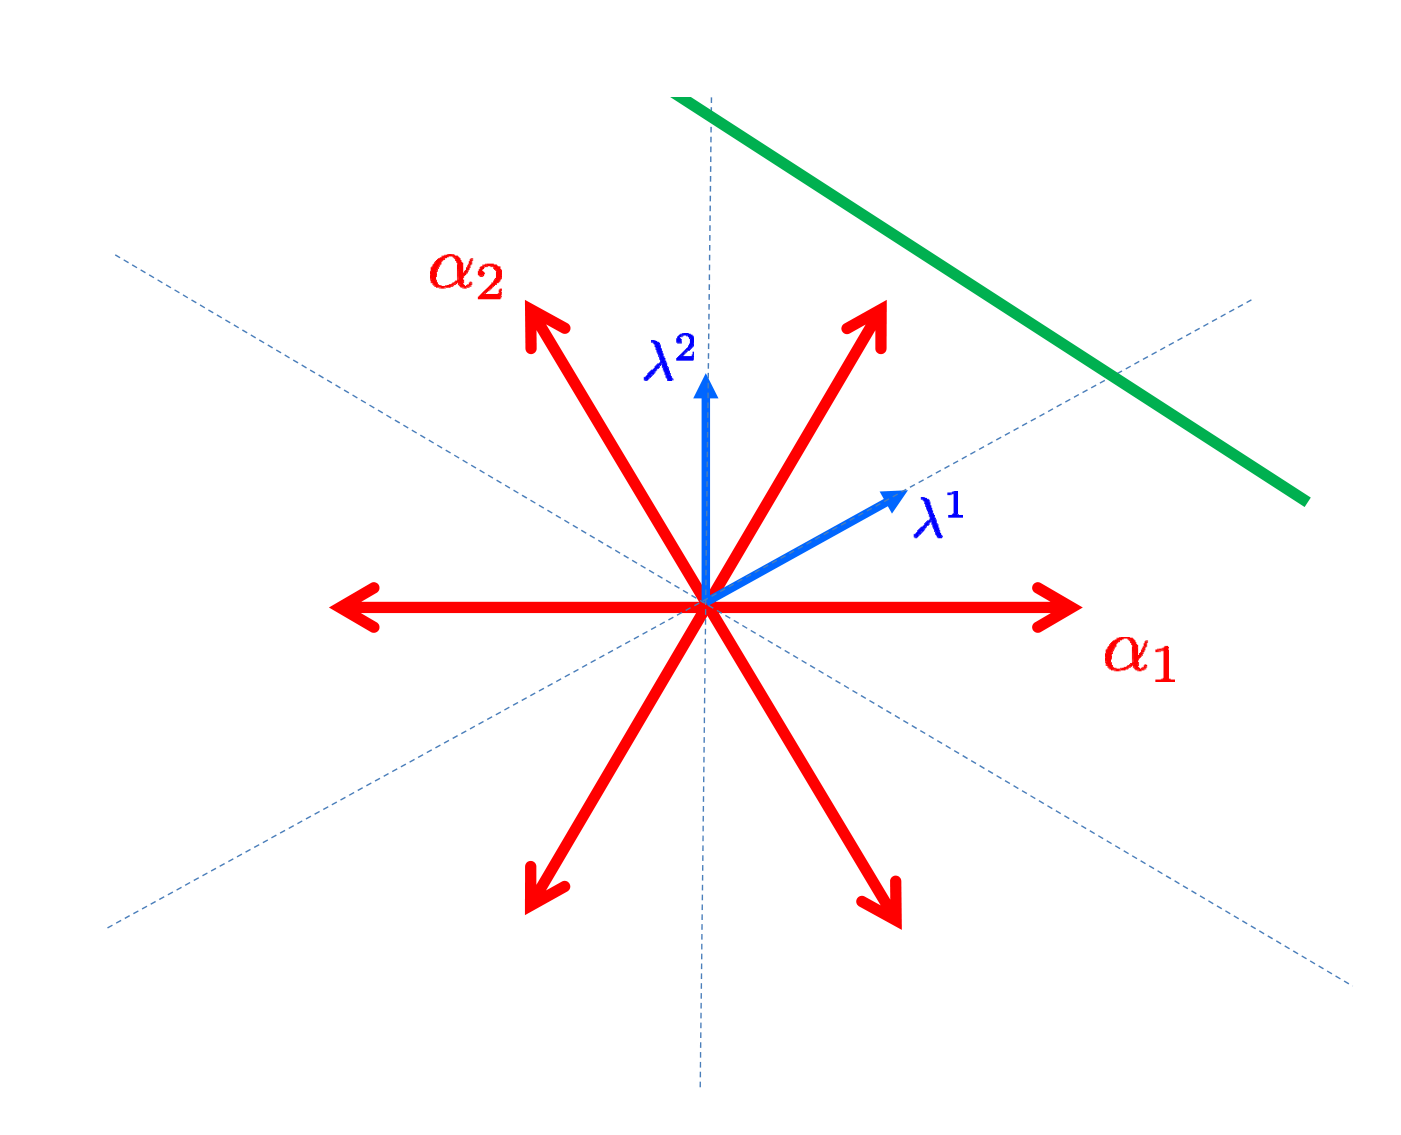
\includegraphics[width=0.62\textwidth]{figures/fig17.png}
  \caption{$SU(3)$ 的根格与权格。图中给出了一组标准的单根 $\alpha_1,\alpha_2$，以及基本权 $\lambda^1,\lambda^2$。基本 Weyl 腔是由这两个权张成的正锥。最高根为 $\theta=\alpha_1+\alpha_2$。粗绿线是某个正整数 $k$ 所对应的直线 $(\lambda,\theta)=k$。仿射 Weyl 腔是区域 $(\lambda,\theta)\le k$，而能级 $k$ 的可积权是权格与基本 Weyl 腔的交集。（原文 Fig.~17，第 129 页）}
  \label{fig:17}
\end{figure}

\subsubsection{可积最高权表示的特征标} % 原文: 4.5.3 Characters of integrable highest weight representations

表示 $V(\lambda)$ 的\emph{特征标}（characters）是
\begin{equation}
  \operatorname{Tr}_{V(\lambda)}q^{L_0}e^{2\pi i\zeta\cdot H_0}
  \tag{4.156}
  \label{eq:4.156}
\end{equation}
其中 $\zeta\in\mathrm{t}^*\otimes\mathbb{C}$，$q=e^{2\pi i\tau}$，$\tau$ 取值于上半平面。
% 原文把 Cartan 子代数记作正体的 $\mathrm{t}$（而非 Fraktur 体的 $\mathfrak{t}$），与 $\mathfrak{g}$、$\widetilde{\mathfrak{g}}$ 的花体形成对照；转写时保持正体。

通过估计各权空间的维数，可以得知这是 $\zeta$ 与 $\tau$ 的整函数。注意：必须把 $L_0$ 计入才能得到有限的表达式。

导出特征标显式的途径有四条：
\begin{enumerate}
  \item 基于 Verma 模构造的代数方法。
  \item 由权重数（weight multiplicities）的递推关系得到的微分方程。
  \item 应用不动点公式与 Borel-Weil-Bott 定理。
  \item 写出相空间路径积分：对在 $G/T$ 上运动的粒子取作用量
  \begin{equation*}
    S\sim\int\langle\lambda,g^{-1}\dot g\rangle-\int dt\,H(g(t)),
  \end{equation*}
  并用驻相法——结果表明驻相法是精确的。对 Weyl 群求和，就是对运动方程的经典解求和。
\end{enumerate}
% 第 4 条把"对 Weyl 群求和"解释为"对经典解求和"，这一步成立的前提是 $G/T$ 上的驻相近似为精确的（等变定位定理）；原文未加证明。

% ===== 原文印刷页 130（PDF p.131）=====

我们只勾勒第 (1) 条途径。Verma 模的特征标是直截了当的，因为它本质上是一个 Fock 空间。抽象地，它可以写成
\begin{equation}
  \frac{e^{\lambda}}{\prod_{\alpha>0}(1-e^{-\alpha})}
  \tag{4.157}
  \label{eq:4.157}
\end{equation}
例如，对 $SU(2)$ 的 $M(2j)$ 我们有
\begin{equation}
  \operatorname{Tr}_{M(2j)}u^{2J_3}=\frac{u^{2j}}{1-u^{-2}}
  \tag{4.158}
  \label{eq:4.158}
\end{equation}
对 $2j\in\mathbb{Z}_{\ge0}$，不可约表示是商 $M(2j)/M(-2j-2)$，因此 $SU(2)$ 的特征标是：
\begin{equation}
\begin{aligned}
  \chi_j(u) &:=\operatorname{Tr}_{V(j)}u^{2J_3}
  =\operatorname{Tr}_{M(2j)}u^{2J_3}-\operatorname{Tr}_{M(-2j-2)}u^{2J_3}\\
  &=\frac{u^{2j}}{(1-u^{-2})}-\frac{u^{-2j-2}}{(1-u^{-2})}
  =\frac{u^{2j+1}-u^{-2j-1}}{u-u^{-1}}
\end{aligned}
  \tag{4.159}
  \label{eq:4.159}
\end{equation}
% 原文 (4.159) 排成单独一行（其编号因此被挤到下一行右侧）；中译本版心较窄，故在第二个等号处折行，编号仍只出现一次。
% [Tutor Note: (4.159) 末式由前式通分得到：两项通分得 $(u^{2j}-u^{-2j-2})/(1-u^{-2})$，再把分子分母同乘 $u$，即得分子 $u^{2j+1}-u^{-2j-1}$、分母 $u-u^{-1}$，可自行验算以免漏掉 $u^{-1}$ 因子。此外 (4.159) 用的是 $u$ 变量，而 (4.168) 之后改用 $y=e^{2\pi iz}$；二者是同一变量 $u=y$，(4.159) 的两项之差正是后文 (4.167) 中 $\Theta_{1,2}-\Theta_{-1,2}$ 的分子，也就是仿射 Weyl 群奇反射 (4.163) 的贡献。]

一般地，对半单的 $\mathfrak{g}$，其不可约表示的特征标是相应 Verma 模特征标的线性组合。利用 Weyl 群的不变性可以证明 Weyl-Kac 特征标公式：
\begin{equation}
  \chi_{\lambda}=\frac{\sum_{w\in W}\epsilon(w)e^{w(\lambda+\rho)-\rho}}{\prod_{\alpha>0}(1-e^{-\alpha})}
  \tag{4.160}
  \label{eq:4.160}
\end{equation}
例如，对 $\widetilde{Lsu(2)}$ 我们有
\begin{equation}
  \operatorname{Tr}_{M(j)}q^{L_0}e^{2\pi i\zeta H_0}
  =\frac{q^{\frac{(j+\frac12)^2-\frac14}{k+2}}e^{2\pi i\zeta(2j)}}
  {(1-e^{-4\pi i\zeta})\prod_{n=1}^{\infty}(1-q^{n})(1-e^{4\pi i\zeta}q^{n})(1-e^{-4\pi i\zeta}q^{n})}
  \tag{4.161}
  \label{eq:4.161}
\end{equation}
分母中的因子分别对应于算符 $J_0^-$、$H_{-n}$、$J_{-n}^+$、$J_{-n}^-$ 作用在最高权向量上的贡献。
% 核对 (4.161) 的 $q$ 指数：$(j+\frac12)^2-\frac14=j(j+1)$，故指数为 $h_j=j(j+1)/(k+2)$，即 $\widehat{su}(2)_k$ 中自旋 $j$ 的最高权态的 $L_0$ 本征值；此处并未减去 $c/24$（$c=3k/(k+2)$），所以 (4.161) 是 Verma 模的迹，与 (4.168) 定义的特征标相差 $q^{-c/24}=q^{-k/(8(k+2))}$。

现在，仿射 Weyl 群一般是 $\Lambda_{weight}\ltimes W$，其中 $W$ 是 $\mathfrak{g}$ 的 Weyl 群。对 $\mathfrak{g}=su(2)$，它就是 $\mathbb{Z}\ltimes\mathbb{Z}_2$，它作用在权上的方式是
\begin{equation}
  j\to j+m(k+2) \qquad m\in\mathbb{Z}
  \tag{4.162}
  \label{eq:4.162}
\end{equation}
对应偶变换，而
\begin{equation}
  j\to -1-j-m(k+2) \qquad m\in\mathbb{Z}
  \tag{4.163}
  \label{eq:4.163}
\end{equation}
对应奇变换。例如：$(J_0^-)^{2j+1}|j\rangle$ 对应于 $m=0$ 的奇 Weyl 反射，而 $(J_{-1}^+)^{k+1-2j}|j\rangle$ 对应于 $m=-1$ 的奇 Weyl 反射，依此类推。

由此我们导出
\begin{equation}
\begin{aligned}
  Tr_{V(j)}\big[q^{L_0}e^{i2\pi z2J_0^3}\big] &= \\
  &= \frac{\sum_m q^{\frac{1}{k+2}\left[(j+\frac12+m(k+2))^2-1/4\right]}
  \left(e^{i4\pi z(j+\frac12+m(k+2))}-e^{-i4\pi z(j+\frac12+m(k+2))}\right)}
  {(e^{2\pi iz}-e^{-2\pi iz})\prod(1-e^{i4\pi z}q^{n})(1-e^{-i4\pi z}q^{n})(1-q^{n})}
\end{aligned}
  \tag{4.164}
  \label{eq:4.164}
\end{equation}
% 原文 (4.164) 左边的 $Tr$ 为斜体，与本页其余公式的正体 $\operatorname{Tr}$ 不一致；照原样转写。又分母的 $\prod$ 未写出指标，应为 $\prod_{n\ge1}$。

% ===== 原文印刷页 131（PDF p.132）=====

对回圈群 $\widetilde{SU(2)}_k$。

现在来了一个漂亮的技巧：对 $j=0,\ k=0$，唯一的幺正不可约表示是平凡表示。因此，分子等于分母。

引入由下式定义的能级 $k$ 的 theta 函数
\begin{equation}
  \Theta_{\mu,k}(z,\tau):=\sum_{n\in\mathbb{Z}}q^{k(n+\mu/(2k))^2}y^{(\mu+2kn)}
  =\sum_{\ell=\mu\operatorname{mod}2k}q^{\ell^2/(4k)}y^{\ell}
  \tag{4.165}
  \label{eq:4.165}
\end{equation}
其中 $y=e^{2\pi iz}$。我们为圆周上粒子引入的 Riemann theta 函数对应于能级 $1/2$。注意：
\begin{equation}
\begin{aligned}
  \Theta_{\mu,k}(\omega,\tau) &= \Theta_{\mu+2ka,k}(\omega,\tau) \qquad a\in\mathbb{Z}\\
  \Theta_{\mu,k}(-\omega,\tau) &= \Theta_{2k-\mu,k}(\omega,\tau)=\Theta_{-\mu,k}(\omega,\tau)
\end{aligned}
  \tag{4.166}
  \label{eq:4.166}
\end{equation}
% (4.165) 第二个等号要求 $\ell\equiv\mu\ (\mathrm{mod}\ 2k)$，故 $\Theta_{\mu,k}$ 只在 $\mu$ 模 $2k$ 的意义下有定义——这正是 (4.166) 第一式的内容。

我们把 $j=0,\ k=0$ 时的分子认作 $\Theta_{1,2}(z,\tau)-\Theta_{-1,2}(z,\tau)$，于是
\begin{equation}
  \Theta_{1,2}(z,\tau)-\Theta_{-1,2}(z,\tau)
  =(e^{2\pi iz}-e^{-2\pi iz})\prod(1-e^{i4\pi z}q^{n})(1-e^{-i4\pi z}q^{n})(1-q^{n})
  =-i\vartheta_1(2z,\tau)
  \tag{4.167}
  \label{eq:4.167}
\end{equation}
接下来是一个概念上重要的步骤。如果我们稍微修改特征标的定义，把它定义为
\begin{equation}
  \chi_j^k(z,\tau):=\operatorname{Tr}_{V(j)}q^{L_0-c/24}e^{2\pi iz(2J_0^3)}
  \tag{4.168}
  \label{eq:4.168}
\end{equation}
特征标就会具有非常漂亮的数学性质。从 Lie 代数理论的角度看这也许显得不自然，但它在物理上有很好的动机：我们减掉的是基态能量。

现在我们可以写出优雅的公式：
\begin{equation}
\begin{aligned}
  \chi_j^k(z,\tau) &:= \operatorname{tr}q^{L_0-c/24}e^{2\pi iz(2J_0^3)}\\
  &= \frac{\Theta_{2j+1,k+2}(z,\tau)-\Theta_{-2j-1,k+2}(z,\tau)}{\Theta_{1,2}(z,\tau)-\Theta_{-1,2}(z,\tau)}\\
  &= q^{(\ell+1)^2/(4(k+2))-1/8}\chi_j(y)+\cdots
\end{aligned}
  \tag{4.169}
  \label{eq:4.169}
\end{equation}
其中 $0\le j\le k/2$，且 $j$ 取半整数。
% [Tutor Note: (4.169) 有三处易错：(i) 第二行分母用 $\Theta_{1,2}-\Theta_{-1,2}$（能级 2、指标 $\pm1$），分子用能级 $k+2$、指标 $\pm(2j+1)$；(ii) 第三行末尾的 $\chi_j(y)$ 是 $SU(2)$ 的**群**特征标（即 (4.159) 的 $\chi_j(u)$ 取 $u=y=e^{2\pi iz}$），与左边的**仿射**特征标 $\chi_j^k$ 同符号但含义不同；(iii) 第三行 $q$ 的指数应为 $h_j-c/24=j(j+1)/(k+2)-k/(8(k+2))$，而原文写的是 $(\ell+1)^2/(4(k+2))-1/8$，其中 $-1/8$ 只是 $-k/(8(k+2))$ 在 $k\to\infty$ 时的极限，故第三行应读作大 $k$ 领头渐近项，一般 $k$ 下需替换。]

\subsubsection{模性质} % 原文: 4.5.4 Modular properties

特征标满足许多漂亮的数学性质。它们给出 \emph{Jacobi 形式}（Jacobi forms）的例子。当特殊化到 $\zeta=0$ 时，它们在 $PSL(2,\mathbb{Z})$ 下构成一个由\emph{模形式}（modular forms）组成的向量。

回忆 $SL(2,\mathbb{Z})$ 是 $SL(2,\mathbb{R})$ 中矩阵元为整数的子群。它由 $S$、$T$ 生成，二者分别在附录 C 的公式 (C.2) 与 (C.3) 中定义。

{\small\itshape ［原文标记：与附录 D 中的公式重复。］}
% [原文待办标记，原文 p.131 页边；作者用 \ensuremath{\clubsuit} 标出的旁注，提示此处与附录 D 的公式重复]

$SL(2,\mathbb{Z})$ 通过
\begin{equation}
  (\tau,z)\to\Big(\frac{a\tau+b}{c\tau+d},\frac{z}{c\tau+d}\Big)
  \tag{4.170}
  \label{eq:4.170}
\end{equation}
作用在 $(\tau,z)$ 上。

% ===== 原文印刷页 132（PDF p.133）=====

注意它在 $\tau$ 上的作用经过 $PSL(2,\mathbb{Z}):=SL(2,\mathbb{Z})/\langle-1\rangle$ 分解。注意 $T:\tau\to\tau+1$，$S:\tau\to-1/\tau$。

利用 Poisson 求和公式，可以验证能级 $k$ 的 theta 函数在 $SL(2,\mathbb{Z})$ 的生成元下的变换规律：
\begin{equation}
  \Theta_{\mu,k}(\omega,\tau+1)=e^{2\pi i\frac{\mu^2}{4k}}\Theta_{\mu,k}(\omega,\tau)
  \tag{4.171}
  \label{eq:4.171}
\end{equation}
\begin{equation}
  \Theta_{\mu,k}(-\omega/\tau,-1/\tau)=(-i\tau)^{1/2}e^{2\pi ik\omega^2/\tau}
  \sum_{\nu=0}^{2k-1}\frac{1}{\sqrt{2k}}e^{2\pi i\frac{\mu\nu}{2k}}\Theta_{\nu,k}(\omega,\tau)
  \tag{4.172}
  \label{eq:4.172}
\end{equation}
由 \eqref{eq:4.172} 可以推出
\begin{equation}
  (\Theta_{1,2}-\Theta_{-1,2})(-z/\tau,-1/\tau)
  =i(-i\tau)^{1/2}e^{4\pi iz^2/\tau}(\Theta_{1,2}-\Theta_{-1,2})(z,\tau)
  \tag{4.173}
  \label{eq:4.173}
\end{equation}
再做一点简短的计算便得到：
\begin{equation}
  \chi_j^{su(2)}(-1/\tau,-z/\tau)=e^{2\pi ikz^2/\tau}
  \sum_{j'=0}^{k/2}S_{jj'}\chi_{j'}^{su(2)}(\tau,z)
  \tag{4.174}
  \label{eq:4.174}
\end{equation}
其中
\begin{equation}
  S_{jj'}=\sqrt{\frac{2}{k+2}}\sin\frac{\pi(2j+1)(2j'+1)}{k+2}.
  \tag{4.175}
  \label{eq:4.175}
\end{equation}
$T$ 的作用容易算出为：
\begin{equation}
  \chi_j^k(\tau+1,z)
  =e^{2\pi i\left(\frac{(\ell+1)^2}{4(k+2)}-\frac18\right)}\chi_j^k(\tau,z)
  =e^{2\pi i\frac{2\ell(\ell+2)-k}{8(k+2)}}\chi_j^k(\tau,z)
  \tag{4.176}
  \label{eq:4.176}
\end{equation}
其中 $\ell=2j$。这两个变换生成模群 $SL(2,\mathbb{Z})$ 的一个幺正表示。
% [Tutor Note: (4.175) 是 $\widehat{su}(2)_k$ 的模 $S$ 矩阵；核对归一化最省事的办法是用 $S^2=\mathbf{1}$ 的实形式（$S$ 对称且 $S^2$ 给出电荷共轭 $\mu\to-\mu$），以及 $j\to k/2-j$ 时 $\sin$ 的对称性。注意 (4.174) 左边变量顺序是 $(-1/\tau,-z/\tau)$，而 (4.168) 中 $z$ 出现在 $e^{2\pi iz(2J_0^3)}$ 里，故必须配合 (4.176) 与 (4.172) 才能得到不含前因子 $e^{2\pi ikz^2/\tau}$ 的"纯"矩阵元；漏掉前因子是常见错误。]

\textbf{注记}

\begin{enumerate}
  \item 一般地，特征标由 Weyl-Kac 特征标公式给出。正如 Weyl 特征标公式可以写成
  \begin{equation}
    \frac{\sum_{w\in W}e^{w(\lambda+\rho)-\rho}}{\sum_{w\in W}e^{w(\rho)-\rho}}
    \tag{4.177}
    \label{eq:4.177}
  \end{equation}
  Weyl-Kac 特征标公式也可以写成完全同样的形式，只需把对 Weyl 群的求和换成对仿射 Weyl 群的求和，并把 $\lambda$、$\rho$ 换成相应的仿射权。我们在公式 (??) 中认出了对仿射 Weyl 群求和的结构：theta 函数来自对 $\mathbb{Z}$ 的求和，而 theta 函数之差来自 $SU(2)$ 的 Weyl 群中那个非平凡的反射。
% [原文待办标记，原文 p.132；"equation (??)" 是作者未填写的交叉引用，从上下文看应指 (4.169)（或与之等价的 (4.164)），此处照原样保留问号]
  \item 一般地可以取 $\lambda=0$，得到分母恒等式：
  \begin{equation}
    \sum_{w\in W}\epsilon(w)e^{w(\rho)}=\prod_{\alpha>0}\big(e^{\frac12\alpha}-e^{-\frac12\alpha}\big)
    \tag{4.178}
    \label{eq:4.178}
  \end{equation}
\end{enumerate}

% ===== 原文印刷页 133（PDF p.134）=====

\begin{enumerate}[start=3]
  \item 在广义 Kac-Moody 代数上，\eqref{eq:4.178} 有许多很有意思的推广。{\small\itshape ［原文标记：此处需要补文献！］}
% [原文待办标记，原文 p.133；原文作 "[NEED CITATIONS HERE!]"]
  \item 事实表明，$G_k$ 的表示论与相应量子群在 $q$ 取适当单位根时的表示论密切相关：
  \begin{equation}
    q=\exp\Big(\frac{2\pi i}{k+h}\Big)
    \tag{4.179}
    \label{eq:4.179}
  \end{equation}
  详见 Fuchs 的书。
  \item 上述故事可以推广到更广的一类二维共形场论，即所谓"有理共形场论"（rational conformal field theories）。
\end{enumerate}

\medskip\noindent\textbf{练习}\quad 仔细解释为什么 $j=k=0$ 的不可约表示是平凡表示。

\noindent 证明 $M(j=0,k=0)/S(j=0,k=0)$ 是一维的。

\medskip\noindent\textbf{练习}\quad 求出 $\widetilde{su(3)}$ 在能级 $k$ 的可积表示，并说明它们在权格上如何分布。

\subsection{WZW 的 Hilbert 空间与单圈配分函数} % 原文: 4.6 The Hilbert Space Of WZW And The One-Loop Partition Function

% 本片段无 \section 级标题（4.6 为 \subsection），故按规范不插入「本节重点」；该小节要点备忘：
% (i) $\mathcal{H}=\oplus_{0\le\lambda\cdot\theta\le k}\overline{V_\lambda}\otimes V_\lambda$ 是 Peter-Weyl 定理的精确类比，每个幺正不可约表示恰好出现一次；
% (ii) 单圈配分函数等于以 $\tau=\theta+i\beta$ 为模参数的平坦环面上的路径积分，$H=L_0+\bar{L}_0-c/12$、$P=L_0-\bar{L}_0$；
% (iii) 微分同胚不变性 + 共形反常下 Weyl 标度贡献为零 $\Rightarrow$ $Z$ 模不变，由 $\chi_\lambda$ 的幺正模表示保证；
% (iv) 存在非对角模不变组合 $\sum N_{j\bar j}\chi_j\overline{\chi_{\bar j}}$（$N$ 非单位矩阵倍数）。

Hilbert 空间与单圈配分函数。

注：大 $k$ 极限：粒子在群 $G$ 上运动。$L^2(G)$ 分解的截断。环面上的共形块。$S$ 矩阵与 $T$ 矩阵。
% 这几行是作者的写作提纲（"Note: ..."），并非完整句子，译文按原样逐句译出、未作展开；它预告了本节的三条主线：大 $k$ 的粒子图像、$L^2(G)$ 分解被截断到 $(\lambda,\theta)\le k$ 的有限多项、以及环面上共形块的 $S$、$T$ 矩阵。

对紧群 $G$，Hilbert 空间具有漂亮的结构。事实证明，Hilbert 空间关于量子 $\widetilde{LG}_L\times\widetilde{LG}_R$ 对称性的分解，把每一个幺正不可约表示都恰好编码一次。因此，它是紧群 Peter-Weyl 定理的完美类比。

我们有
\begin{equation}
  \mathcal{H}=\oplus_{0\le\lambda\cdot\theta\le k}\overline{V_{\lambda}}\otimes V_{\lambda}
  \tag{4.180}
  \label{eq:4.180}
\end{equation}
其中
\begin{equation}
  0\le\lambda\cdot\theta\le k
  \tag{4.181}
  \label{eq:4.181}
\end{equation}
而 $\theta$ 是 $\mathfrak{g}$ 的最高根。对 $SU(2)$ 能级 $k$ 的模型，我们特别有：

% ===== 原文印刷页 134（PDF p.135）=====

\begin{equation}
  \mathcal{H}=\oplus_{0\le j\le k/2}\overline{V_j}\otimes V_j
  \tag{4.182}
  \label{eq:4.182}
\end{equation}
特征标的模性质现在得到了漂亮的解释。考虑配分函数：
\begin{equation}
  Z=\operatorname{Tr}_{\mathcal{H}}e^{-2\pi\beta H+2\pi i\theta P}
  =\operatorname{Tr}_{\mathcal{H}}q^{L_0-c/24}\bar{q}^{\bar{L}_0-c/24}
  \tag{4.183}
  \label{eq:4.183}
\end{equation}
其中
\begin{equation}
  H=L_0+\bar{L}_0-c/12
  \tag{4.184}
  \label{eq:4.184}
\end{equation}
\begin{equation}
  P=L_0-\bar{L}_0
  \tag{4.185}
  \label{eq:4.185}
\end{equation}
而
\begin{equation}
  \tau=\theta+i\beta
  \tag{4.186}
  \label{eq:4.186}
\end{equation}
于是
\begin{equation}
  Z=\sum_{\lambda}\overline{\chi_{\lambda}(\tau,0)}\chi_{\lambda}(\tau,0)
  \tag{4.187}
  \label{eq:4.187}
\end{equation}
{\small\itshape ［原文标记：这里真的需要补上与平坦规范场的耦合！！！］}
% [原文待办标记，原文 p.134 页边；作者用 \ensuremath{\clubsuit} 标出的旁注 "REALLY NEED TO ADD COUPLING TO FLAT GAUGE FIELDS HERE!!!"，提示应在 (4.187) 处加入与平坦背景规范场的耦合]

% [Tutor Note: 原 PDF 第 134 页的 Figure 18 为空白占位框，图形内容在原稿中缺失，仅存图注；此处按原图注翻译并保留图号，以免后文图号错位。]
\begin{figure}[htbp]
  \centering
  \MissingFigureNote
  \caption{取迹在 $z=\sigma+it$ 平面上所诱导的等同（identifications）。我们先沿欧氏时间传播 $\beta$，然后在等同状态之前，沿 $\sigma$ 方向作一个 $2\pi\theta$ 的平移扭转。（原文 Fig.~18，第 134 页）}
  \label{fig:18}
\end{figure}
% [排版说明：原 PDF 中 Fig.~18 的图形本身缺失，页面上只余图注与留白，figures/fig18.png 为对应的空白裁片，按原样插入以保留编号与位置]

配分函数 \eqref{eq:4.183} 可以解释为平坦环面上的路径积分，该环面的模参数为 $\tau$，如图 18 所示。我们将在第 2.2.12 节看到，$\tau$ 上的模变换等价于环面上非平凡微分同胚的作用。

另一方面，配分函数必须是微分同胚不变的。Weyl 标度对配分函数的影响为零，这是由于共形反常，并且背景度规是平坦的。因此，配分函数必须是模不变的。这一点得以实现，是因为 $\chi_{\lambda}$ 按模群的幺正表示变换。

\textbf{注记}：存在不同的模不变特征标组合。也就是说，可以找到非负整数 $N_{j,\bar{j}}$，它们不正比于单位矩阵，使得
\begin{equation}
  \sum_{j,\bar{j}}N_{j\bar{j}}\chi_{j}\overline{\chi_{\bar{j}}}
  \tag{4.188}
  \label{eq:4.188}
\end{equation}
% (4.188) 中的 $\bar{j}$ 表示右移（反全纯）侧的指标，与左移的 $j$ 独立取值，二者各自遍历 $0\le j\le k/2$，不可混为同一个指标；$N_{j\bar j}$ 取单位矩阵即退化为对角组合 (4.187)。
